\documentclass[aspectratio=169,handout]{beamer}
\usepackage[utf8x]{inputenc}
\usepackage{tikz}
\usepackage[european]{circuitikz}
\usepackage[ngerman]{babel}
\usepackage{marvosym}
\usepackage{booktabs}

% This file contains configuration shared between main file and figures

\usepackage{pifont}
\usepackage{xspace}
\DeclareUnicodeCharacter{2460}{\ding{172}\xspace}
\DeclareUnicodeCharacter{2461}{\ding{173}\xspace}

\usepackage{tikz}

\definecolor{HB9UFblue}{RGB}{0,61,165}
\definecolor{HB9UFred}{HTML}{ED135A}

\newcommand{\Ohm}{$\Omega$\xspace}


\newcommand{\uline}[1]{%
  \tikz[baseline=(todotted.base)]{
      \node[inner sep=1pt,outer sep=0pt] (todotted) {#1};
      \draw[color=HB9UFblue,thick] (todotted.south west) -- (todotted.south east);
  }%
}%
                           
\newcommand{\udash}[1]{%
  \tikz[baseline=(todotted.base)]{
      \node[inner sep=1pt,outer sep=0pt] (todotted) {#1};
      \draw[dashed,color=HB9UFred,thick] (todotted.south west) -- (todotted.south east);
  }%
}%


\usepackage{pifont}
\usepackage{xspace}
\DeclareUnicodeCharacter{2460}{\ding{172}\xspace}
\DeclareUnicodeCharacter{2461}{\ding{173}\xspace}

\usetikzlibrary{arrows,positioning}

\usepackage{pgfplots}
\usepackage{pgfpages}
%\setbeameroption{show notes on second screen=right}
%\pgfpagesuselayout{3 on 1 with notes}[a4paper,border shrink=3mm]
%\setbeameroption{show notes on second screen=right}
%\setbeamertemplate{note page}{\pagecolor{yellow!5}\insertnote}\usepackage{palatino}

\usetheme{metropolis}

\makeatletter
\setbeamertemplate{title page}{
  \begin{minipage}[b][\paperheight]{\textwidth}
    \vfill%
    \vspace{-1cm}%
    \ifx\inserttitle\@empty\else\usebeamertemplate*{title}\fi
    \ifx\insertsubtitle\@empty\else\usebeamertemplate*{subtitle}\fi
    \usebeamertemplate*{title separator}
    \ifx\beamer@shortauthor\@empty\else\usebeamertemplate*{author}\fi
    \ifx\insertdate\@empty\else\usebeamertemplate*{date}\fi
    \ifx\insertinstitute\@empty\else\usebeamertemplate*{institute}\fi
    \ifx\inserttitlegraphic\@empty\else\usebeamertemplate*{title graphic}\fi
    \vfill
    \vspace*{1mm}
  \end{minipage}
}
\makeatother
\makeatletter
\pgfdeclareshape{cornernumber}{
  \inheritsavedanchors[from=rectangle] % this is nearly a rectangle
  \inheritanchorborder[from=rectangle]
  \inheritanchor[from=rectangle]{center}
  \inheritanchor[from=rectangle]{north}
  \inheritanchor[from=rectangle]{south}
  \inheritanchor[from=rectangle]{west}
  \inheritanchor[from=rectangle]{east}
  \inheritanchor[from=rectangle]{north west}
  \backgroundpath{% this is new
    % store lower right in xa/ya and upper right in xb/yb
    \southwest \pgf@xa=\pgf@x \pgf@ya=\pgf@y
    \northeast \pgf@xb=\pgf@x \pgf@yb=\pgf@y
    % construct main path
    \pgfsetcornersarced{\pgfpoint{5pt}{5pt}}
    \pgfpathmoveto{\pgfpoint{\pgf@xa}{\pgf@ya}}
    \pgfpathlineto{\pgfpoint{\pgf@xa}{\pgf@yb}}
    \pgfsetcornersarced{\pgfpoint{0pt}{0pt}}
    \pgfpathlineto{\pgfpoint{\pgf@xb}{\pgf@yb}}
    \pgfpathlineto{\pgfpoint{\pgf@xb}{\pgf@ya}}
    \pgfpathclose
 }
}
\makeatother

\title{NanoVNA Workshop}
\author{UHF-Gruppe der USKA, HB9UF}
\date{1. Juli 2023}
% FIXME: Titelbild
%\titlegraphic{\noindent\makebox[\textwidth]{\includegraphics[width=\paperwidth]{titelbild}}}
%\titlegraphic{\includegraphics[width=\textwidth]{titelbild}}


\begin{document}
\frame[plain]{\titlepage}

\begin{frame}{Ablauf}
    \begin{enumerate}
        \item Einleitung und Organisatorisches
        \item Was ist im Säckli? (Was ist nicht im Säckli?)
        \item Was ist ein VNA?
        \item Einstellungen: Frequenz und Trace-Format
        \item S11: Reflexionsmessung mit Kalibrierung
        \item S21: Transmissionsmessung mit Kalibrierung
        \item Postenlauf
        \item Smith-Diagramm und Abschluss
    \end{enumerate}
    \textbf{Pausen nach Belieben während des Postenlaufs.}
\end{frame}

%\begin{frame}{Die UHF-Gruppe der USKA -- Wer sind wir?}
%    % FIXME
%\end{frame}

\begin{frame}{Ziele von heute}
    \begin{itemize}
        \item NanoVNA kennenlernen.
        \item Möglichst viel mit dem eigenen Gerät messen.
        \item Was ist good practice und was sind die Grenzen des Gerätes?
        \item Diskussion der Messresultate unter den Teilnehmenden.
        \item Interessante Gespräche, Austausch etc.
    \end{itemize}
\end{frame}

\begin{frame}{Was ist ein VNA? ``Vector Network Analyzer''}
          \begin{center}
              \begin{tikzpicture}[text width=6em, text centered,, node distance=8em]
                  \tikzstyle{box}=[draw,rounded corners=3pt,minimum height=3em]
                  %\node[box] (p1) {\sf\Large{Port ① \small{(CH0)}}};
                  \node[box] (p1) {\sf\Large{Port 1 \small{(CH0)}}};
                  \node[box,right=of p1] (dut) {\sf\Large{DUT}};
    %             \node[box,right=of dut] (p2) {\sf\Large{Port ② \small{(CH1)}}};
                  \draw[-stealth',thick,transform canvas={yshift=2mm}] (p1) -- node[above] {\sf Stimulus} (dut);
                  \draw[-stealth',thick,transform canvas={yshift=-2mm}] (dut) -- node[below]{\sf Reflexion} (p1);

                  \onslide<3->\node[box,right=of dut] (p2) {\sf\Large{Port 2 \small{(CH1)}}};
                  \onslide<3->\draw[-stealth',thick] (dut) -- node[above] {\sf Transmission} (p2);
              \end{tikzpicture}
          \end{center}

      \vfill

      \begin{enumerate}
          \onslide<2->{\item Reflexionsmessungen (\textbf{S11}, S22)}
          \onslide<3->{\item Transmissionsmessungen (\textbf{S21}, S12)}
          \onslide<4->{\item Vektoriell}
      \end{enumerate}

      \vfill

      DUT: Device Under Test (``Prüfling'')
\end{frame}

\begin{frame}{Postenlauf}
    \textbf{Posten A:} Reflexionsmessungen passiver Bauteile

    \textbf{Posten B:} Transmissionsmessungen an Filtern

    \textbf{Posten C:} Impedanztransformatoren und Mantelwellensperren (``Baluns'')

    \textbf{Posten D:} Antennen

\end{frame}


\begin{frame}{Impedanznetzwerke (1)}
        \begin{circuitikz}
        \draw (0,0) to[battery=$U_Q$] (0,-4)
              (0,0) to[short] (3,0) to[R,a=50~$\Omega$] (3,-2) to[short,-o] (5,-2)
              (3,-2) to[R,a=50~$\Omega$,*-*] (3,-4) to[short,-o] (5,-4)
              (3,-4) to[short,-*] (0,-4) node[ground] {};
        \draw[-stealth',shorten >=3mm,shorten <=3mm] (5,-2) -- node[right]{$U_L$} (5,-4);
     \end{circuitikz}
    \begin{tikzpicture}
        \begin{axis}[
            xmin=0, xmax=10,
            ymin=-1.25,ymax=1.25,
            ylabel={Spannung / V},
            grid=both,
            xlabel={Zeit / ns},
            yticklabels={-1,-.5,0,.5,1},
            xtick = {0,2.5,5,7.5,10},
            ytick = {-1,-0.5,0,0.5,1},
            height=4cm,
            width=7.5cm,
            major grid style={black!10},
        ]
        \pgfplotsset{every y tick label/.append style={font=\tiny}}
        \only<2>{\addplot [mark=none,samples=100,domain=0:10,color=HB9UFblue,thick] {0.5} node[below,pos=0.45] {$U_L$};}
        \addplot [mark=none,samples=100,domain=0:10,color=HB9UFred,dashed,thick] {1} node[below,pos=0.33] {$U_Q$};
        \end{axis}
    \end{tikzpicture}

\end{frame}

\begin{frame}{Impedanznetzwerke (2)}
        \begin{circuitikz}
        \draw (0,0) to[sinusoidal voltage source=$U_Q$] (0,-4)
              (0,0) to[short] (3,0) to[R,a=50~$\Omega$] (3,-2) to[short,-o] (5,-2)
              (3,-2) to[R,a=50~$\Omega$,*-*] (3,-4) to[short,-o] (5,-4)
              (3,-4) to[short,-*] (0,-4) node[ground] {};
        \draw[-stealth',shorten >=3mm,shorten <=3mm] (5,-2) -- node[right]{$U_L$} (5,-4);
     \end{circuitikz}
    \begin{tikzpicture}
        \begin{axis}[
            xmin=0, xmax=10,
            ymin=-1.25,ymax=1.25,
            ylabel={Spannung / V},
            grid=both,
            xlabel={Zeit / ns},
            yticklabels={-1,-.5,0,.5,1},
            xtick = {0,2.5,5,7.5,10},
            ytick = {-1,-0.5,0,0.5,1},
            height=4cm,
            width=7.5cm,
            major grid style={black!10}
        ]
        \pgfplotsset{every y tick label/.append style={font=\tiny}}
        \only<2>{\addplot [mark=none,samples=100,domain=0:10,color=HB9UFblue,thick] {0.5*sin(3600*x)} node[below,pos=0.45] {$U_L$};}
        \addplot [mark=none,samples=100,domain=0:10,color=HB9UFred,dashed,thick] {sin(3600*x)} node[above,pos=0.45] {$U_Q$};
        \end{axis}
    \end{tikzpicture}
\end{frame}

\begin{frame}{Impedanznetzwerke (3)}
        \begin{circuitikz}
        \draw (0,0) to[sinusoidal voltage source=$U_Q$] (0,-4)
              (0,0) to[short] (3,0) to[R,a=50~$\Omega$] (3,-2) to[short,-o] (5,-2)
              (3,-2) to[L,a=80~nH,*-*] (3,-4) to[short,-o] (5,-4)
              (3,-4) to[short,-*] (0,-4) node[ground] {};
        \draw[-stealth',shorten >=3mm,shorten <=3mm] (5,-2) -- node[right]{$U_L$} (5,-4);
     \end{circuitikz}
    \begin{tikzpicture}
        \begin{axis}[
            xmin=0, xmax=10,
            ymin=-1.25,ymax=1.25,
            ylabel={Spannung / V},
            grid=both,
            xlabel={Zeit / ns},
            yticklabels={-1,-.5,0,.5,1},
            xtick = {0,2.5,5,7.5,10},
            ytick = {-1,-0.5,0,0.5,1},
            height=4cm,
            width=7.5cm,
            major grid style={black!10}
        ]
        \pgfplotsset{every y tick label/.append style={font=\tiny}}
        \only<2>{\addplot [mark=none,samples=100,domain=0:10,color=HB9UFblue,thick] {0.7*sin(3600*x+45)} node[below,pos=0.45] {$U_L$};}
        \addplot [mark=none,samples=100,domain=0:10,color=HB9UFred,dashed,thick] {sin(3600*x)} node[above,pos=0.45] {$U_Q$};
        \end{axis}
    \end{tikzpicture}
\end{frame}

\begin{frame}{Impedanz: Kombination aus Wirk- und Blindwiderstand}
    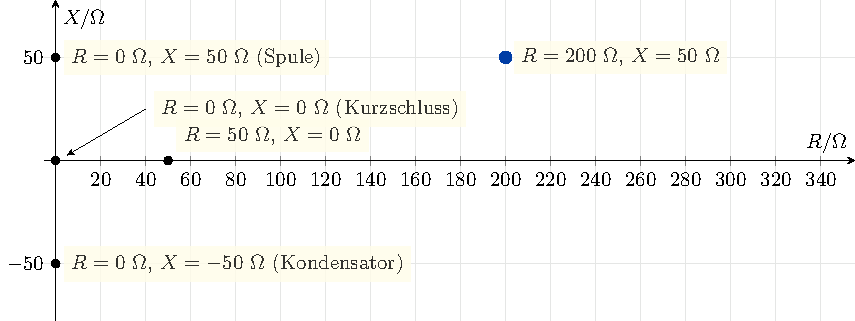
\includegraphics{../skript/figures/complex_plane/complex_plane.pdf}
\end{frame}

\begin{frame}{Smith Diagramm: Impedanzen in einem transformierten Koordinatensystem}
    \begin{center}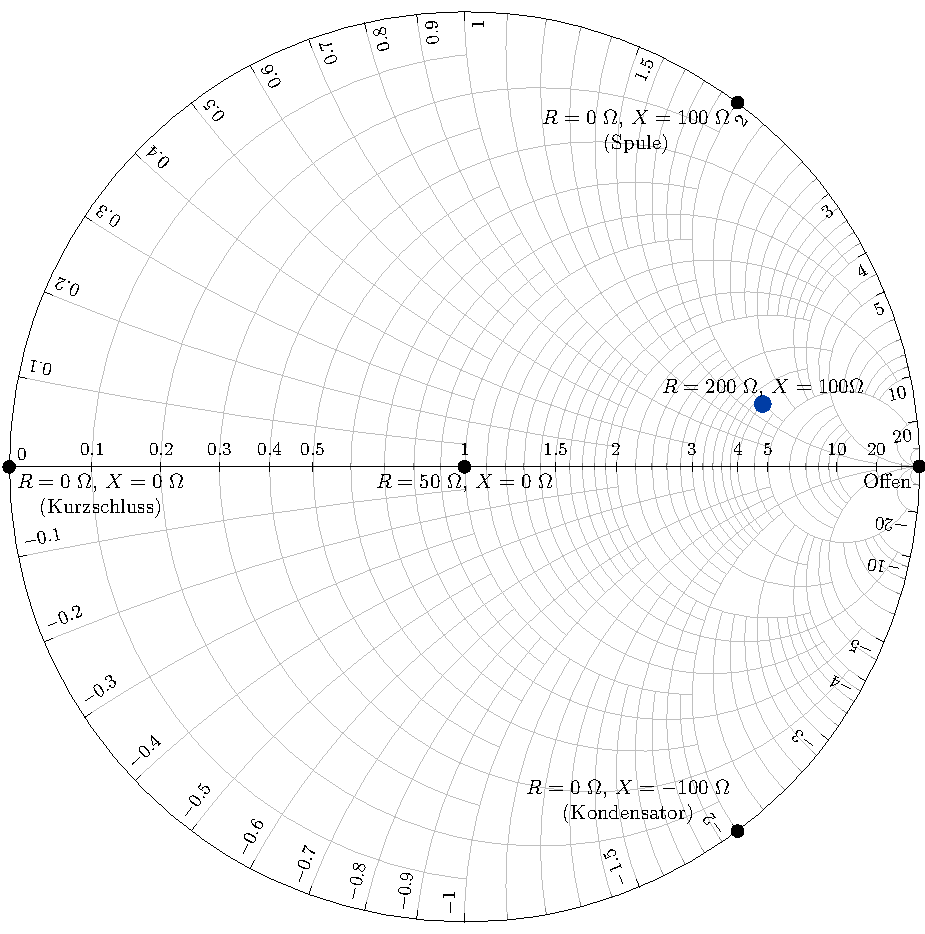
\includegraphics[height=0.9\textheight]{../skript/figures/complex_smith/complex_smith.pdf}\end{center}
\end{frame}
\end{document}
